\documentclass{article}
\title{ファイナンス基礎 — 金利・現在価値・ポートフォリオ}
\author{TeX 図書館}

\begin{document}

\section{この教科書のために — 金融の共通言語}

「1 年後の 100 万円」と「今の 100 万円」は同じ価値ではありません。\textbf{時間と金利}を通してお金の価値を翻訳するのがファイナンスの基本技術で、債券・不動産・企業価値・退職計画はすべてこの翻訳の応用です。

この教科書は『投資の数学』(期待値・ケリー・資金管理)の直後の位置にあり、そこで学んだ確率の道具を\textbf{お金の時間価値}と\textbf{ポートフォリオ理論}に接続します。

\section{複利 — 世界最大の発明と呼ばれる力}

元本 \(C\) を年利 \(r\) で \(n\) 年運用すると(年 1 回の利払いを再投資):
\[ C(1 + r)^n \]
単利なら \(C(1 + rn)\) ですが、複利は\textbf{利子が利子を生む}ので差が指数的に開きます。

\begin{figure}[h]
\centering
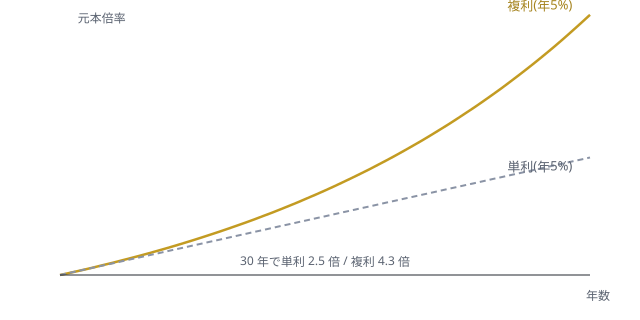
\includegraphics[width=0.8\textwidth]{figures/compound.svg}
\caption{年利 5\% の単利と複利。30 年で単利 2.5 倍に対し複利は 4.3 倍になる。}
\end{figure}

\begin{quote}
\textbf{【72 の法則】}\ 「金利 \(r\)(\%)で元本が 2 倍になる年数 \(\approx 72/r\)」。年 6\% なら 12 年で 2 倍、年 3\% なら 24 年。計算機なしで複利の規模感を掴む古典的な道具です(正確には \(\ln 2 / \ln(1+r) \approx 72/r\) という近似)。
\end{quote}

\begin{quote}
\textbf{【演習】}\ 年利 5\% の複利で元本が 3 倍になる年数を求めよ(対数計算)。72 の法則の推定とも比較せよ。
\end{quote}

\textbf{解答の指針:}\ \((1.05)^n = 3\) より \(n = \ln 3 / \ln 1.05 \approx 22.5\) 年。72 の法則(72/5 = 14.4 年は「2 倍」)を 3 倍に外挿すると 14.4 × 1.585 ≈ 22.8 年でよく合う。

\section{現在価値 — 未来のお金を今の値段に翻訳する}

金利 \(r\) のとき、「1 年後の \(C\) 円」の\textbf{現在価値}は
\[ \mathrm{PV} = \frac{C}{1 + r} \]
「今 \(C/(1+r)\) 円を運用すれば 1 年後に \(C\) 円になる」から等価です。\(n\) 年後なら \(C/(1+r)^n\)。\textbf{遠い将来のお金ほど、金利が高いほど}現在価値は小さくなります。

\begin{quote}
\textbf{【例】}\ 「10 年後に 2000 万円受け取る権利」と「今 1200 万円」。割引率 5\% なら権利の現在価値は \(2000/1.05^{10} \approx 1228\) 万円——わずかに権利が有利。\textbf{割引率の選択が結論を左右する}のが現在価値計算の本質です。
\end{quote}

\begin{quote}
\textbf{【演習】}\ 「毎年 100 万円を 10 年間受け取る年金」の現在価値を、割引率 5\% で求めよ(等比数列の和)。
\end{quote}

\textbf{解答の指針:}\ \(\sum_{t=1}^{10} \frac{100}{1.05^t} = 100 \times \frac{1 - 1.05^{-10}}{0.05} \approx 772\) 万円(年金現価係数 7.72)。

\section{債券 — 金利と価格が逆に動く仕組み}

\textbf{債券}は「元本を貸して、利子を受け取り、満期に返してもらう」契約です。その価格は\textbf{将来キャッシュフローの現在価値の合計}で決まります:
\[ P = \sum_{t=1}^{N} \frac{\text{クーポン}}{(1+y)^t} + \frac{\text{額面}}{(1+y)^N} \]

ここから重要な性質が従います:\textbf{市場金利 \(y\) が上がると、債券価格は下がる}(割引率が上がれば現在価値は減る)。逆も同様。債券は「金利の逆」。この機械的な関係が、金利上昇局面で債券が売られる理由のすべてです。

\begin{quote}
\textbf{【例】}\ 額面 100 円・クーポン年 2\%・残存 10 年の債券。市場金利が 2\% なら価格は 100 円。金利が 3\% に上がると価格は \(\sum 2/1.03^t + 100/1.03^{10} \approx 91.4\) 円に下落。\textbf{残存年数が長いほど下落が大きい}(将来の割り引き期間が長いため)。
\end{quote}

\begin{quote}
\textbf{【演習】}\ 残存 1 年の債券と残存 30 年の債券、金利上昇に対してどちらが価格の変動が大きいか、現在価値の式から説明せよ。
\end{quote}

\textbf{解答の指針:}\ 30 年債。額面の現在価値 \(100/(1+y)^N\) の \(y\) に対する感度は \(N\) に比例して大きくなる。これが「デュレーションが長いほど金利リスクが大きい」の正体。

\section{リスクとリターン — 分散投資の数理}

\begin{quote}
\textbf{【定理:分散効果】}\ 相関係数 \(\rho < 1\) の 2 資産に半分ずつ投資すると、ポートフォリオの分散は
\[ V = \frac{1}{4}(V_1 + V_2 + 2\rho\sqrt{V_1 V_2}) \]
となり、\textbf{個々のリスクの平均より小さくなる}。\(\rho = -1\) ならリスクを完全に消せる。
\end{quote}

「互いに違うものに分けて持つと、全体の揺れが個々の揺れの平均より小さい」——この一点が分散投資の数理的正体です。『統計学入門』の \(V[X+Y] = V[X] + V[Y] + 2\,\mathrm{Cov}\) の共分散項が小さいことがすべてです。

\begin{quote}
\textbf{【演習】}\ 標準偏差 20\% の資産 A と 20\% の資産 B に半分ずつ投資したときのポートフォリオの標準偏差を、\(\rho = 1, 0.5, 0, -1\) の各場合で計算せよ。
\end{quote}

\textbf{解答の指針:}\ 分散 \(= \frac{1}{4}(0.04 + 0.04 + 2\rho \times 0.04)\)。標準偏差は \(\rho = 1\) で 20\%、0.5 で約 17.3\%、0 で約 14.1\%、−1 で 0\%。相関の低さこそが資産。

\section{ポートフォリオ理論 — 効率的フロンティア}

リスクとリターンを平面上に置くと、「同じリスクで最大リターン、同じリターンで最小リスク」な組合せの集合は曲線を描きます。これが\textbf{効率的フロンティア}です。

\begin{itemize}
\item \textbf{無リスク資産}とリスク資産を混ぜる配分は、直線(\textbf{資本配分線, CAL})を描く
\item CAL とフロンティアが接する点が\textbf{最も効率的なリスク資産の組み合わせ}で、あとは無リスク資産との配合だけを変えればよい
\item 「どのリスク水準まで行くか」は個人の許容次第で、\textbf{どの資産ミックスかは理論が決める}——この分離が\textbf{分離定理}です
\end{itemize}

\begin{quote}
\textbf{【演習】}\ 無リスク金利 1\%、リスク資産の期待リターン 6\%・標準偏差 20\% のとき、ポートフォリオ標準偏差 10\% を目指す配分と期待リターンを求めよ。
\end{quote}

\textbf{解答の指針:}\ リスク資産配分 \(w = 10/20 = 0.5\)。期待リターン \(= 0.5 \times 1\% + 0.5 \times 6\% = 3.5\%\)。

\section{配当・インフレ・実質リターン}

\begin{itemize}
\item \textbf{配当利回り} = 年配当 ÷ 株価。配当金は受け取り時の税引き後で再投資される点で、複利の燃料になる
\item \textbf{実質リターン} = \((1 + r) / (1 + \pi) - 1 \approx r - \pi\)(\(\pi\) はインフレ率)。名目 5\%・インフレ 3\% なら実質は約 2\%
\item \textbf{インフレは現金への静かな課金}で、年 3\% なら 24 年で購買力が半減する(72 の法則)
\end{itemize}

\begin{quote}
\textbf{【演習】}\ 名目リターン 6\%・インフレ 2\% のとき、30 年後の 100 万円の実質購買力(現在の金額に換算)を求めよ。
\end{quote}

\textbf{解答の指針:}\ 実質リターン約 3.92\% で成長: \(100 \times (1.06/1.02)^{30} \approx 326\) 万円(現在価値換算)。\textbf{名目 5.74 倍でも実質は 3.26 倍}——インフレの重み。

\section{行動の罠 — 理論と実行の間}

ファイナンス理論は「それでよい」を教えますが、実行は人間です。代表的な行動バイアス:
\begin{enumerate}
\item \textbf{損失回避}: 利益は早売りし、損失は持ち続ける(プロスペクト理論)
\item \textbf{近年バイアス}: 直近の成績を過大評価し、 highs の後で買う
\item \textbf{過信バイアス}: 自分の情報が市場より優れていると信じる。『投資の数学』第 5 節の「推定の信頼性」と直結
\item \textbf{Herding(群集行動)}: みんなが買うから買う。バブルの燃料
\end{enumerate}

防御は\textbf{ルール化}です。積立・リバランス・配分の上限を事前に機械的に決めておくことが、理論を実行に移すための工学的対策です。

\begin{quote}
\textbf{【演習】}\ 「下がったら損切り、上がったら利確しを自動化する」というルールの長所・短所を、損失回避バイアスとの関係で述べよ。
\end{quote}

\textbf{解答の指針:}\ 長所 = 感情の介入を排除し損失を小さく保つ。短所 = 統計的に有利な局面(一時的下落後の回復)も機械的に手放す。ルール化は「感情の除去」であり「勝ちの保証」ではない。

\section{おわりに — 翻訳の技術}

この教科書で手に入れた翻訳機: 複利(§2)、現在価値(§3)、債券価格(§4)、分散効果(§5)、効率的フロンティア(§6)、実質リターン(§7)。そして理論を実行に移す行動設計(§8)。

次の一歩は『株式投資の基礎』(企業の価値をどう見るか)、『オプションの数学入門』(派生商品の価格)、そして退職計画としての『個人財務の設計』です。

\begin{quote}
\textbf{【総合演習】}
\begin{enumerate}
\item 年 7\% の複利で元本 4 倍になる年数を 72 の法則で概算し、対数計算と比較せよ。
\item 標準偏差 15\%・相関 0.3 の 2 資産に等分したポートフォリオの標準偏差を求めよ。
\item 名目 4\%・インフレ 1\% の実質リターンを求めよ。
\end{enumerate}
\end{quote}

\textbf{解答の指針:}\ 1. 72/7 ≈ 10.3 年(2 倍)→ 4 倍は 2 回分で約 20.6 年。対数計算 \(\ln 4/\ln 1.07 \approx 20.5\) 年で一致。2. 分散 \(= \frac{1}{4}(0.0225 + 0.0225 + 2 \times 0.3 \times 0.0225) = 0.014625\)、標準偏差約 12.1\%。3. \(1.04/1.01 - 1 \approx 2.97\%\)(近似では 3\%)。

\end{document}
